\chapter{European Spallation Source and beam diagnostic devices}
\chaptermark{European Spallation Source and beam diagnostic devices}
\cleardoublepage

\minitoc
\section{Introduction}
\begin{refsection}
  \label{ch2:Introduction}
  This thesis deals about the design of non-invasive ionization profilers for the ESS proton beam. To produce neutrons, the European Spallation Source (ESS) is be based on one of the most powerful linear proton accelerators ever built. Therefore, the beam diagnostic is an important part of the project to insure the safety of the machine during the commissioning and the operation.

  This chapter gives an overall vision of the ESS project. The different elements of the accelerator will be briefly detailed from the source to the target. In addition, some neutron instruments foreseen at ESS and their applications will be illustrated.

  The second part of the chapter focuses on beam diagnostic devices and their diversity. An exhaustive list of beam diagnostics is not possible and so only few of them are presented here. The chapter concludes with the state of the art of non-invasive profilers based on the ionization of residual gas.

  \section{European Spallation Source}
  The European Spallation Source (ESS) will be the future neutron source. The source is currently under construction in Lund, Sweden. The objective of ESS is clear: ESS will be the brightest pulsed neutron source in the world and give to Europe a modern flagship neutron source as the ILL was.

  ESS can be roughly summarized in 3 parts: a powerful linear accelerator, a large tungsten target and a multitude of neutron scattering instruments. Each of these elements represents a technological breakthrough in their respective fields.

  Fig. \ref{chap3:fig:ESS_pulse} underlines the difference between in terms of brightness \footnote{The plot does not have have the same scale if power or neutron flux are considered}. compared to existing sources.
  \begin{figure}[!ht]
  \begin{center}
    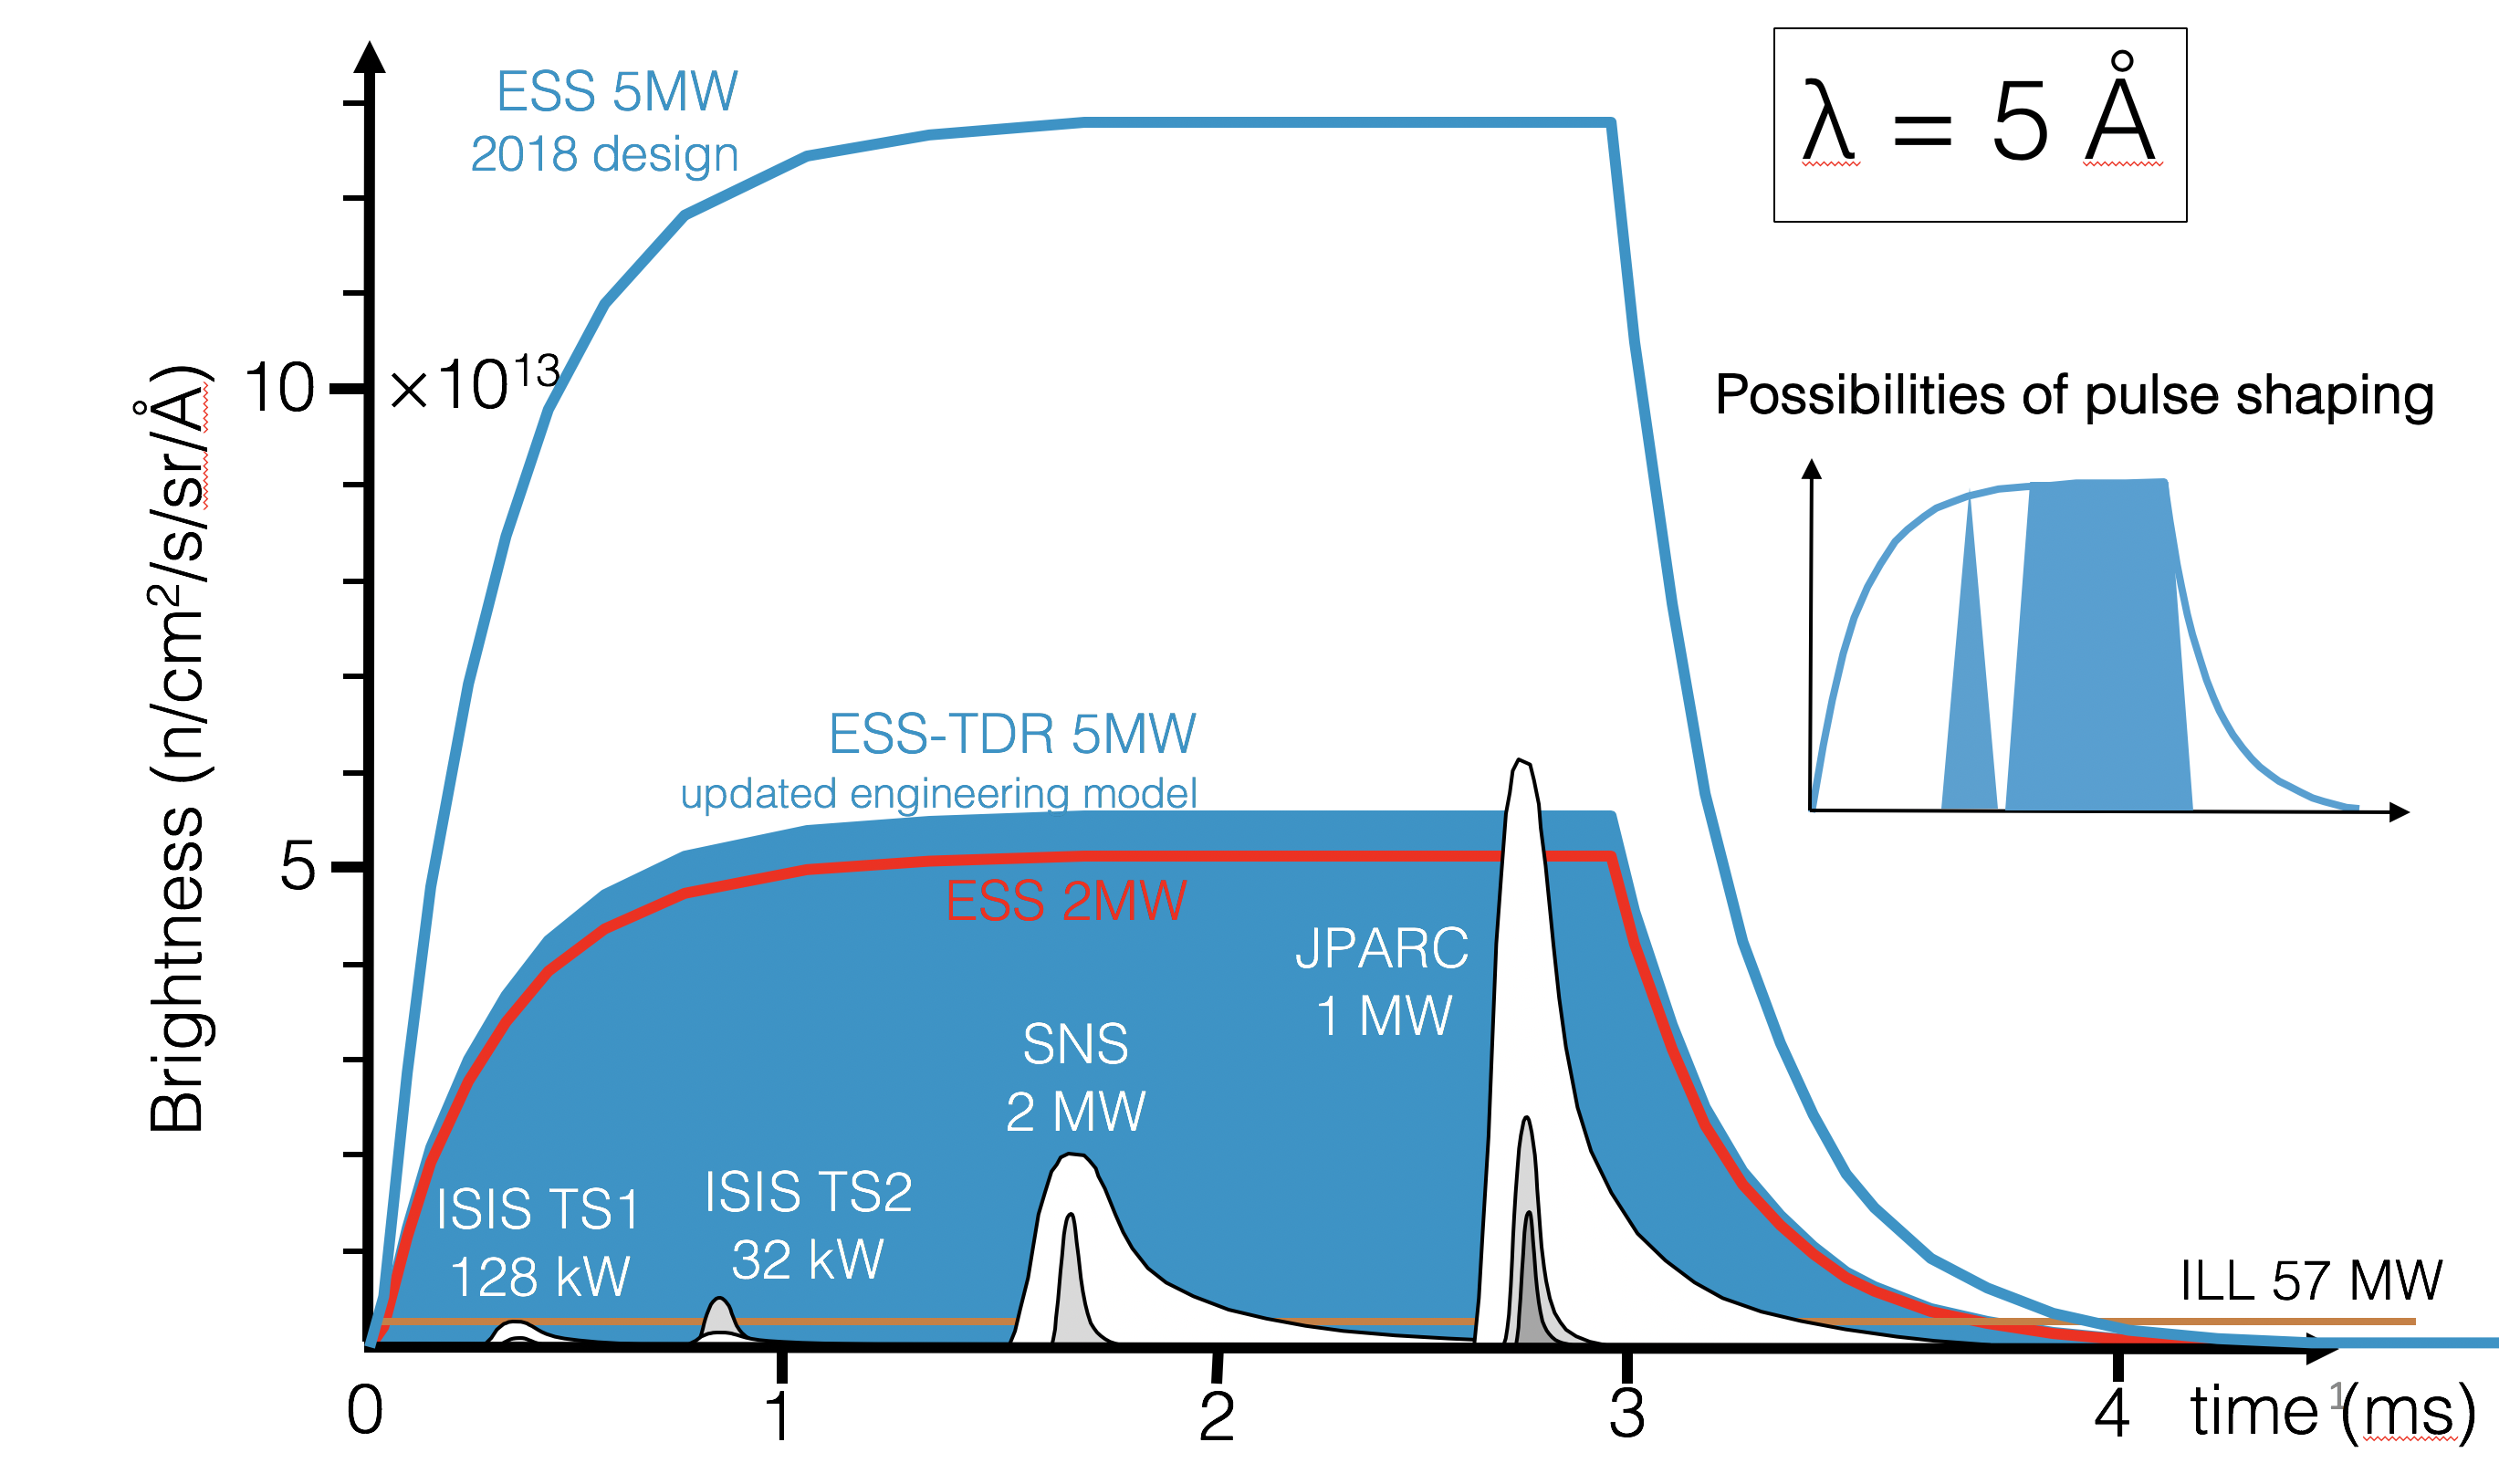
\includegraphics[width=\textwidth]{02_BeamDiag/figures/fig000_ESS_pulse}

  \end{center}
  \caption[ESS neutron source brightness compared to others existing neutron sources]{ESS neutron source brightness compared to others existing neutron sources.}
  \label{chap3:fig:ESS_pulse}
\end{figure}


  \section{ESS collaboration and ESS activities at CEA/IRFU}

  ESS is a very large project based on an international collaboration of many research Institutes. Today, the collaboration includes more than 140 institutes from 15 different countries with more than 40 European in kind agreements. France is very implicated in the ESS project, particularly through two research organizations: the French National Centre for Scientific Research (\acrshort{cnrs}) and the French Alternative Energies and Atomic Energy Commission (\acrshort{cea}).

  CEA is a key player in research, development and innovation in four main areas: defence and security, nuclear and renewable energies, technological research for industry and fundamental research. The Institute for Research on the Fundamental laws of the Universe (\acrshort{irfu}) is one of institute attached to the fundamental research division of CEA. IRFU brings together three scientific disciplines, astrophysics, nuclear physics and particle physics. IRFU develops as well the associated technological required by the cutting-edge research.

  \section{Accelerator basics}

  \section{ESS accelerator}
  The proton linear accelerator (LINAC or linac) of ESS is represented synthetically in Fig. \ref{chap2:fig:ESS_acc}.
  The total length from the source to the target is about $600\,\mathrm{m}$ and $356\,\mathrm{m}$ are dedicated to the acceleration. The first part accelerates the beam up to $90\,\mathrm{MeV}$ by mean of conventional room temperature RF cavities. Then a cold part using superconducting cavities cooled with liquid helium is used to reach the highest energies.

  \begin{figure}[!ht]
	\begin{center}
		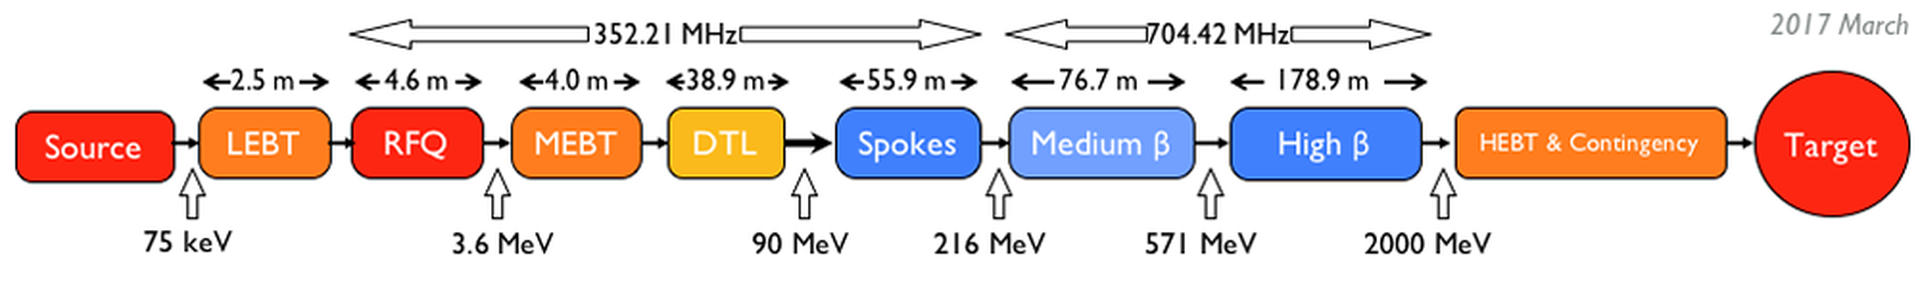
\includegraphics[width=\textwidth]{02_BeamDiag/figures/fig000_ESS_acc}
	\end{center}
	\caption[A simplified representation of the ESS linac]{A simplified representation of the ESS linac. Blue blocks represent superconducting cavities where IPMs will be installed.}
	\label{chap:}
\end{figure}


  Table \ref{chap2:tab:ess_charac} summarizes the most important characteristics of the ESS linac. The particularities of ESS compared to other sources of spallation are its very long pulse and its high current. The average beam power is $5\,\mathrm{MW}$ and the peak power is $125\,\mathrm{MW}$, making ESS one of the most powerful proton accelerators in the world.

  \begin{table}[ht]
  \centering
  \caption[ESS nominal conditions]
  {ESS nominal conditions.}
  \label{chap2:ess_charac}
  \begin{tabular}{ll}
    \toprule
    Characteristic    & Value                  \\
    \midrule
    Energy            & $2\,\mathrm{GeV}$      \\
    Current           & $62.5\,\mathrm{mA}$    \\
    Pulse duration    & $2.86\,\mathrm{ms}$    \\
    Power             & $5\,\mathrm{MW}$       \\
    Repetition rate   & $14\,\mathrm{Hz}$      \\
    Duty cycle        & $4\,\mathrm{\%}$       \\
    Radio Frequencies & $352.21\,\mathrm{MHz}$ \\
                      & $704.42\,\mathrm{MHz}$ \\
    \bottomrule
  \end{tabular}
\end{table}

  In the next sections the role of each of the accelerator blocks is described in few words.

  \subsection{Ion source and Low Energy Beam Transport}
  The source is the first stage of any accelerators, it creates and extracts the plasma. An Electron Cyclotron Resonance (\acrshort{ecr}) source is a type of sources particularly suitable for the production of plasma of mono specie at high intensity \cite{nicke2012}. An ECR source is based on the superposition of a magnetic field and a RF wave. In a magnetic field the electrons orbit around the magnetic field lines with a frequency defined by:
  \begin{equation}
    \omega_{e} = \frac{eB}{m_{e}}
  \end{equation}
  By injecting a powerful RF wave of the same frequency, the electrons will enter into resonance and reach sufficient energy to ionize the medium and create a plasma. In an ECR source the plasma is confined by the magnetic field. Then, a series of electrodes placed at very high potential extract the plasma from the confinement chamber. At the source output, the beam has an energy close to $100\,\mathrm{keV}$, for instance the ESS source accelerates
  proton to $75\,\mathrm{keV}$.

  At low energies the plasma has a strong space charge and is therefore very divergent. The low energy beam transport line (\acrshort{lebt}) contains the space charge by using solenoids, and optimize the injection of the plasma into the first accelerating cavity.
  Fig. \ref{chap2:fig:LEBT_ESS} outlines the source and the LEBT of ESS. An iris allows to finely adjust the beam current and a Faraday cage is able to measure current at the iris output and completely stop the beam. This line also contains diagnostics that check the quality of the beam before the injection into the RFQ.

  The \acrshort{infn} Catania was in charge of the design and production of the source and the LEBT. CEA/IRFU was involved in two diagnostics: a Doppler Shift Unit \cite{Thomas:IPAC2017-MOPVA037} and an Allison scanner\cite{Tuske:IPAC2017-MOPAB023}. The source was delivered to ESS and commissioned in 2018.

  \begin{figure}[!ht]
	\begin{center}
		\includegraphics[width=\textwidth]{example-image-a}
	\end{center}
	\caption[]{}
	\label{chap:}
\end{figure}


  \subsection{Radio Frequency Quadrupole}
  The principle of the Radio Frequency Quadrupole (RFQ) was imagined in the 1970s in Russia by I. M. Kapchinskiy and V. Tepliakov. The method has quickly become popular and indispensable in very intense accelerators since it is still the most efficient method for bunching and accelerating particles at low energies.

  At these energies, the space charge is so high that the beam divergence is enormous and must be compensated. A RFQ behaves as a sequence of focusing and defocusing elements that can contain the space charge. RF waves are propagated on four poles, usually vanes (Fig. \ref{chap2:fig:RFQ_c}) or rods, with opposite amplitude between each pole (Fig. \ref{chap2:fig:RFQ_a}). The RF variation allows to successively focus in one direction (and defocus in the other direction). A mechanical modulation of the vanes introduces a longitudinal electric field that will accelerate the particles (Fig. \ref{chap2:fig:RFQ_b}). The roles of the RFQ are:
  \begin{itemize}
    \item contains and focuses the beam.
    \item structures the beam into small bunches.
    \item accelerates the particles.
  \end{itemize}

  \begin{figure}[!ht]
  \centering
  \begin{subfigure}[t]{0.3\textwidth}
    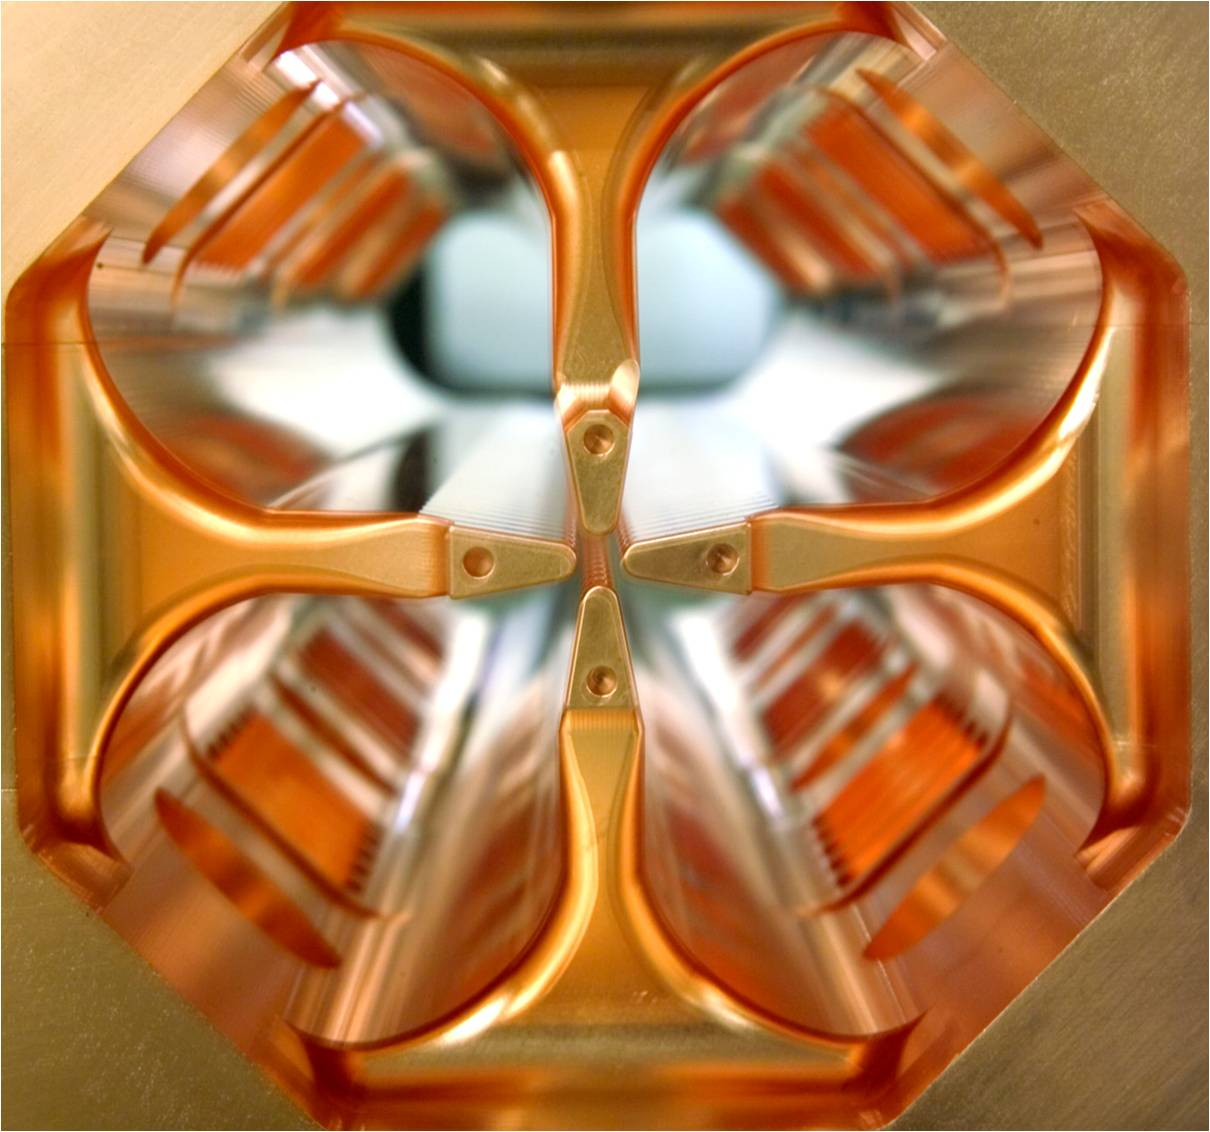
\includegraphics[width=\textwidth]{02_BeamDiag/figures/fig000_RFQ_c}
    \caption[The four copper vanes of a RFQ]{The four copper vanes (poles) of a RFQ.}
    \label{chap2:fig:RFQ_c}
  \end{subfigure}
  ~
  \begin{subfigure}[t]{.3\textwidth}
    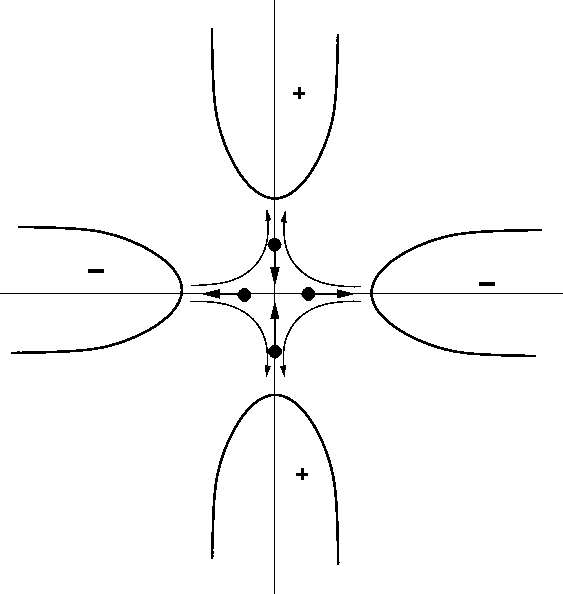
\includegraphics[width=\textwidth]{02_BeamDiag/figures/fig000_RFQ_a}
    \caption{Cut view of the transverse field.}
    \label{chap2:fig:RFQ_a}
  \end{subfigure}
  ~
  \begin{subfigure}[t]{0.3\textwidth}
    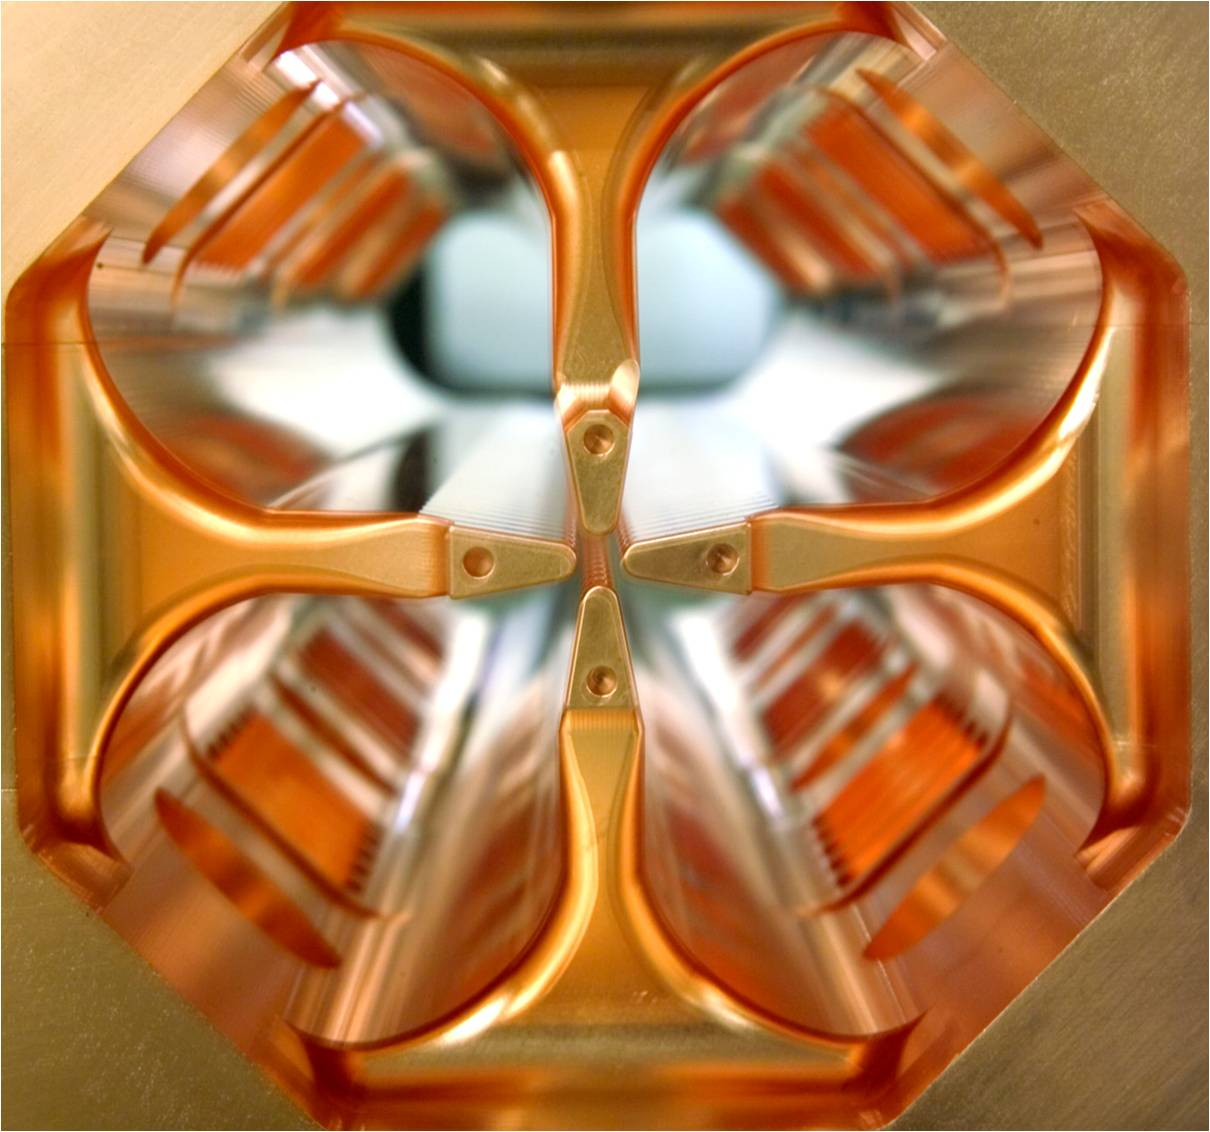
\includegraphics[width=\textwidth]{02_BeamDiag/figures/fig000_RFQ_b}
    \caption[Longitudinal modulation leading to an accelerating field]{Longitudinal modulation leading to an accelerating field \cite{Lombardi:1005049}.}
    \label{chap2:fig:RFQ_b}
  \end{subfigure}

  \caption[An RFQ structure bunches, focuses and accelerates charged particles by means of four poles that modulate the RF wave.]{An RFQ structure bunches, focuses and accelerates charged particles by means of four poles that modulate the RF wave.}
  \label{chap2:fig:RFQ}
\end{figure}


  Simulations of such device are complicated required specific codes to compute the propagation of the RF waves and the transport of particles inside the RFQ \cite{Duperrier2000}. As well, the conception of this type of cavities is extremely technical, for instance the tolerance on the mechanical structures of the vanes is in the order of micrometers whereas the whole RFQ structure often exceeds meters.

  The CEA/IRFU is in charge of the construction of the ESS RFQ \cite{ChirpazIPAC2016} which accelerates the proton beam at the source exit from $75\,\mathrm{keV}$ up to $3.6\,\mathrm{MeV}$ and bunches them with a $352.21\,\mathrm{MHz}$ frequency.

  \subsection{Medium Energy Beam Transport and Drift Tube Linac}
  % TODO: Mettre la référence pour les bunchers
  The medium energy beam transport (\acrshort{mebt}) is located just downstream of the RFQ and contains beam optical elements, buncher cavities and beam diagnostics allowing beam characterization and correction. Fig. \ref{chap2:fig:MEBT} shows a block view of the MEBT and its different elements. Most diagnostics will be presented later in the chapter and a table of abbreviations is available at the end of the thesis. The MEBT has been developed by the ESS-Bilbao team.

  \begin{figure}[!ht]
	\begin{center}
		\includegraphics[width=\textwidth]{example-image-a}
	\end{center}
	\caption[]{}
	\label{chap:}
\end{figure}


  The MEBT prepares the beam for the injection in the Drift Tube Linacs (\acrshort{dtl})\footnote{Sometime, the structure is referred as Alvarez Drift Tube Linac}.
  A DTL cavity is a cylindrical standing waves resonant structure. It uses coaxial cylinders (drift tubes) fixed at one end of support tubes. The acceleration occurs in the gaps between two cylinders. The cylinders are also designed to shield the field for particles during the deceleration phase. The length of these drift tubes is related to the velocity of the particles and increases along the structure. Permanent quadrupole magnet are encapsulated within the coaxial cylinders allowing a  radial focussing of the beam.

  At ESS, the DTL are designed to accelerate beam from $3.62\,\mathrm{MeV}$ to $90\,\mathrm{MeV}$. The ESS DTLs have similar design to the Linac4 DTLs. The DTLs are separated in five DTL tanks containing between 61 to 23 drift tubes. Fig. \ref{} presents some pictures of the ESS DTLs.

  %\begin{figure}[!ht]
	\begin{center}
		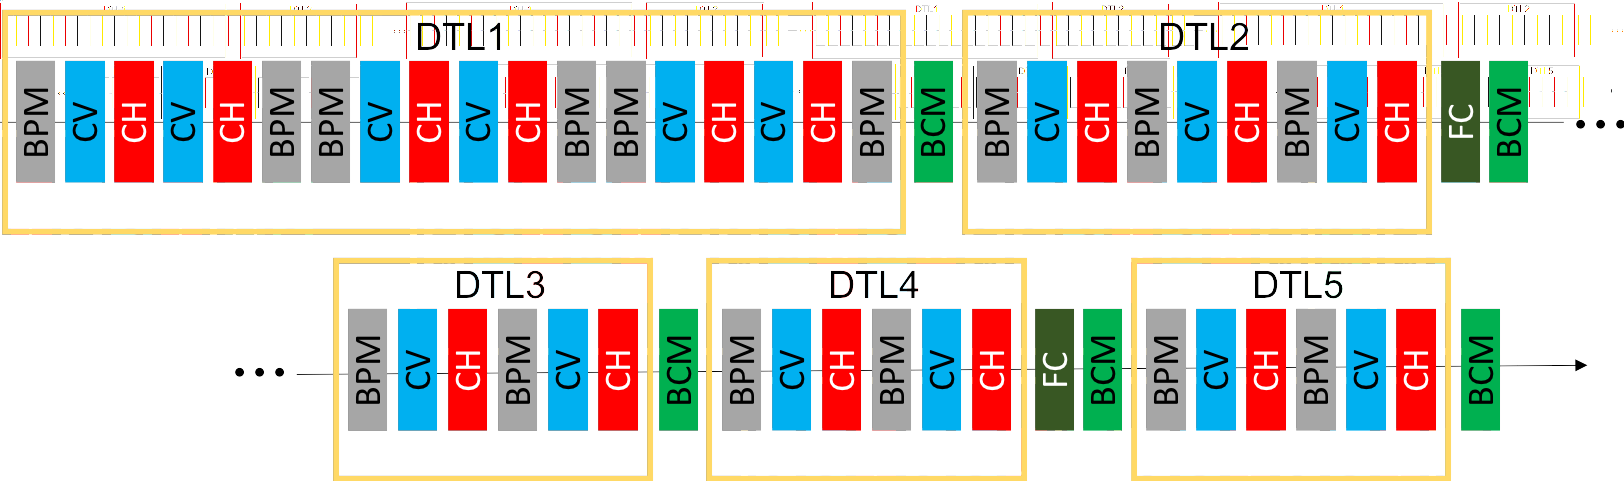
\includegraphics[width=\textwidth]{02_BeamDiag/figures/fig000_DTL}
	\end{center}
	\caption[Building blocks of the MEBT]{Building blocks of the MEBT.}
	\label{chap2:fig:DTL}
\end{figure}

  \subsection{Superconducting cavities}
  The DTL are not optimized beyond 100 MeV because the length of drift tube becomes too long. Two solutions can be considered: increase the accelerating field or increase radio frequency. However, both solutions are technically difficult to implement for long pulsed beam. Indeed, losses in the cavities become very high leading to inefficient acceleration and heating the cavities. The use of superconducting RF cavities overcomes these issues. These superconducting cavities act as perfect conductors when the transition temperature of the superconductor is reached: $9.2\,\mathrm{K}$ for niobium.

  The cooling of these cavities is done by liquid helium system working at $4.13\,\mathrm{K}$, enclosed in a tank with thermal shielding with circuitry for the cooling of cavities, couplers, magnets. The assembly process of such cryomodules must be done in clean conditions and a particle free environment (ISO-5 cleanrooms). A defect on surface or a contamination lead to a loss of the superconductivity capability locally, increasing the RF losses and temperature in this area: a quench.
  As well superconducting cavities are very affected by field emissions.

  Our devices will be installed between two cryomodules, and therefore must be compliant with the constraints imposed by the use of superconducting cavities at ESS. The CEA/IRFU is responsible for the design and integration of medium and high beta cryomodules. Fig. \ref{chap2:fig:ESS_cryo} pictures one elliptical cryomodule.

  \begin{figure}[!ht]
	\begin{center}
		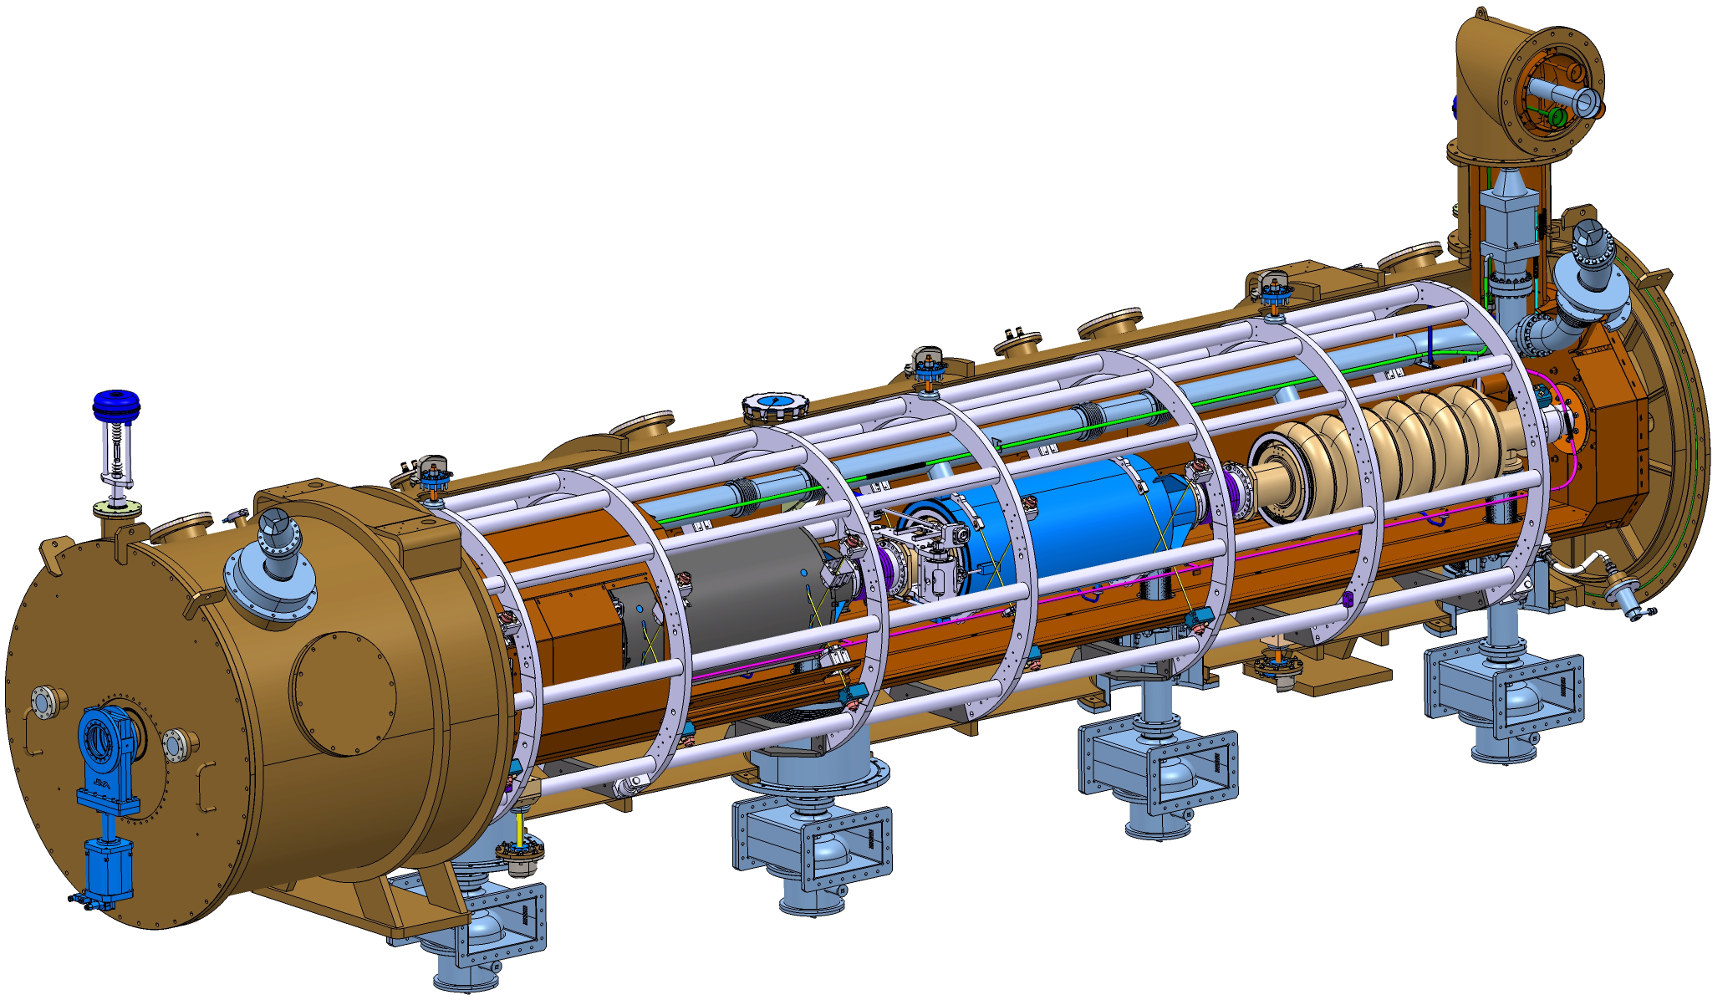
\includegraphics[width=\textwidth]{02_BeamDiag/figures/fig000_cryo_a2}
	\end{center}
	\caption[ESS medium beta elliptical cavities cryomodule]{ESS medium beta elliptical cavities cryomodule.}
	\label{chap2:fig:ESS_cryo}
\end{figure}


  \section{Transport lines and target}
  The protons are then transported in a high-energy beam transport (\acrshort{hebt}) line to the target \footnote{The target is at a different ground level compare to the acclerator.}. A beam dump will be also used during the commissioning phase of the accelerator. The HEBT contains beam diagnostics and beam optic elements that prepare the beam for impacting on the target.

  The ESS target should be designed to maximize the spallation phenomenon and sustain the 5MW beam power. Two technologies are commonly use for spallation targets:
  \begin{itemize}
    \item Solid targets with active cooling (ISIS, SINQ).
    \item Liquid targets with liquid recirculation (SNS, JSNS).
  \end{itemize}
  The solution chosen by ESS is a solid target wheel with a diameter of $2.3\,\mathrm{m}$. The wheel will rotate at $23.33\,\mathrm{rpm}$. The wheel is composed of more than $7000$ small tungsten bricks giving a total weight around 5 tons. The bricks are cooled with liquid helium. The design of the target requires extensive thermal and mechanical studies. All these activities and the manufacturing of the target, as well as many other systems around the target, are under the responsibility of ESS-Bilbao.

  The neutron flux is maximized by means of moderator-reflectors and thermalized by different water and liquid $H_{2}$ moderators. The neutron emission is more or less uniform over the 42 neutron ports around the target. The target moderators and all other systems (engine, cooling etc.) are contained in a shielded structure: the monolith. The monolith is visible in Fig. \ref{chap2:fig:target}.

  \begin{figure}[!ht]
	\begin{center}
		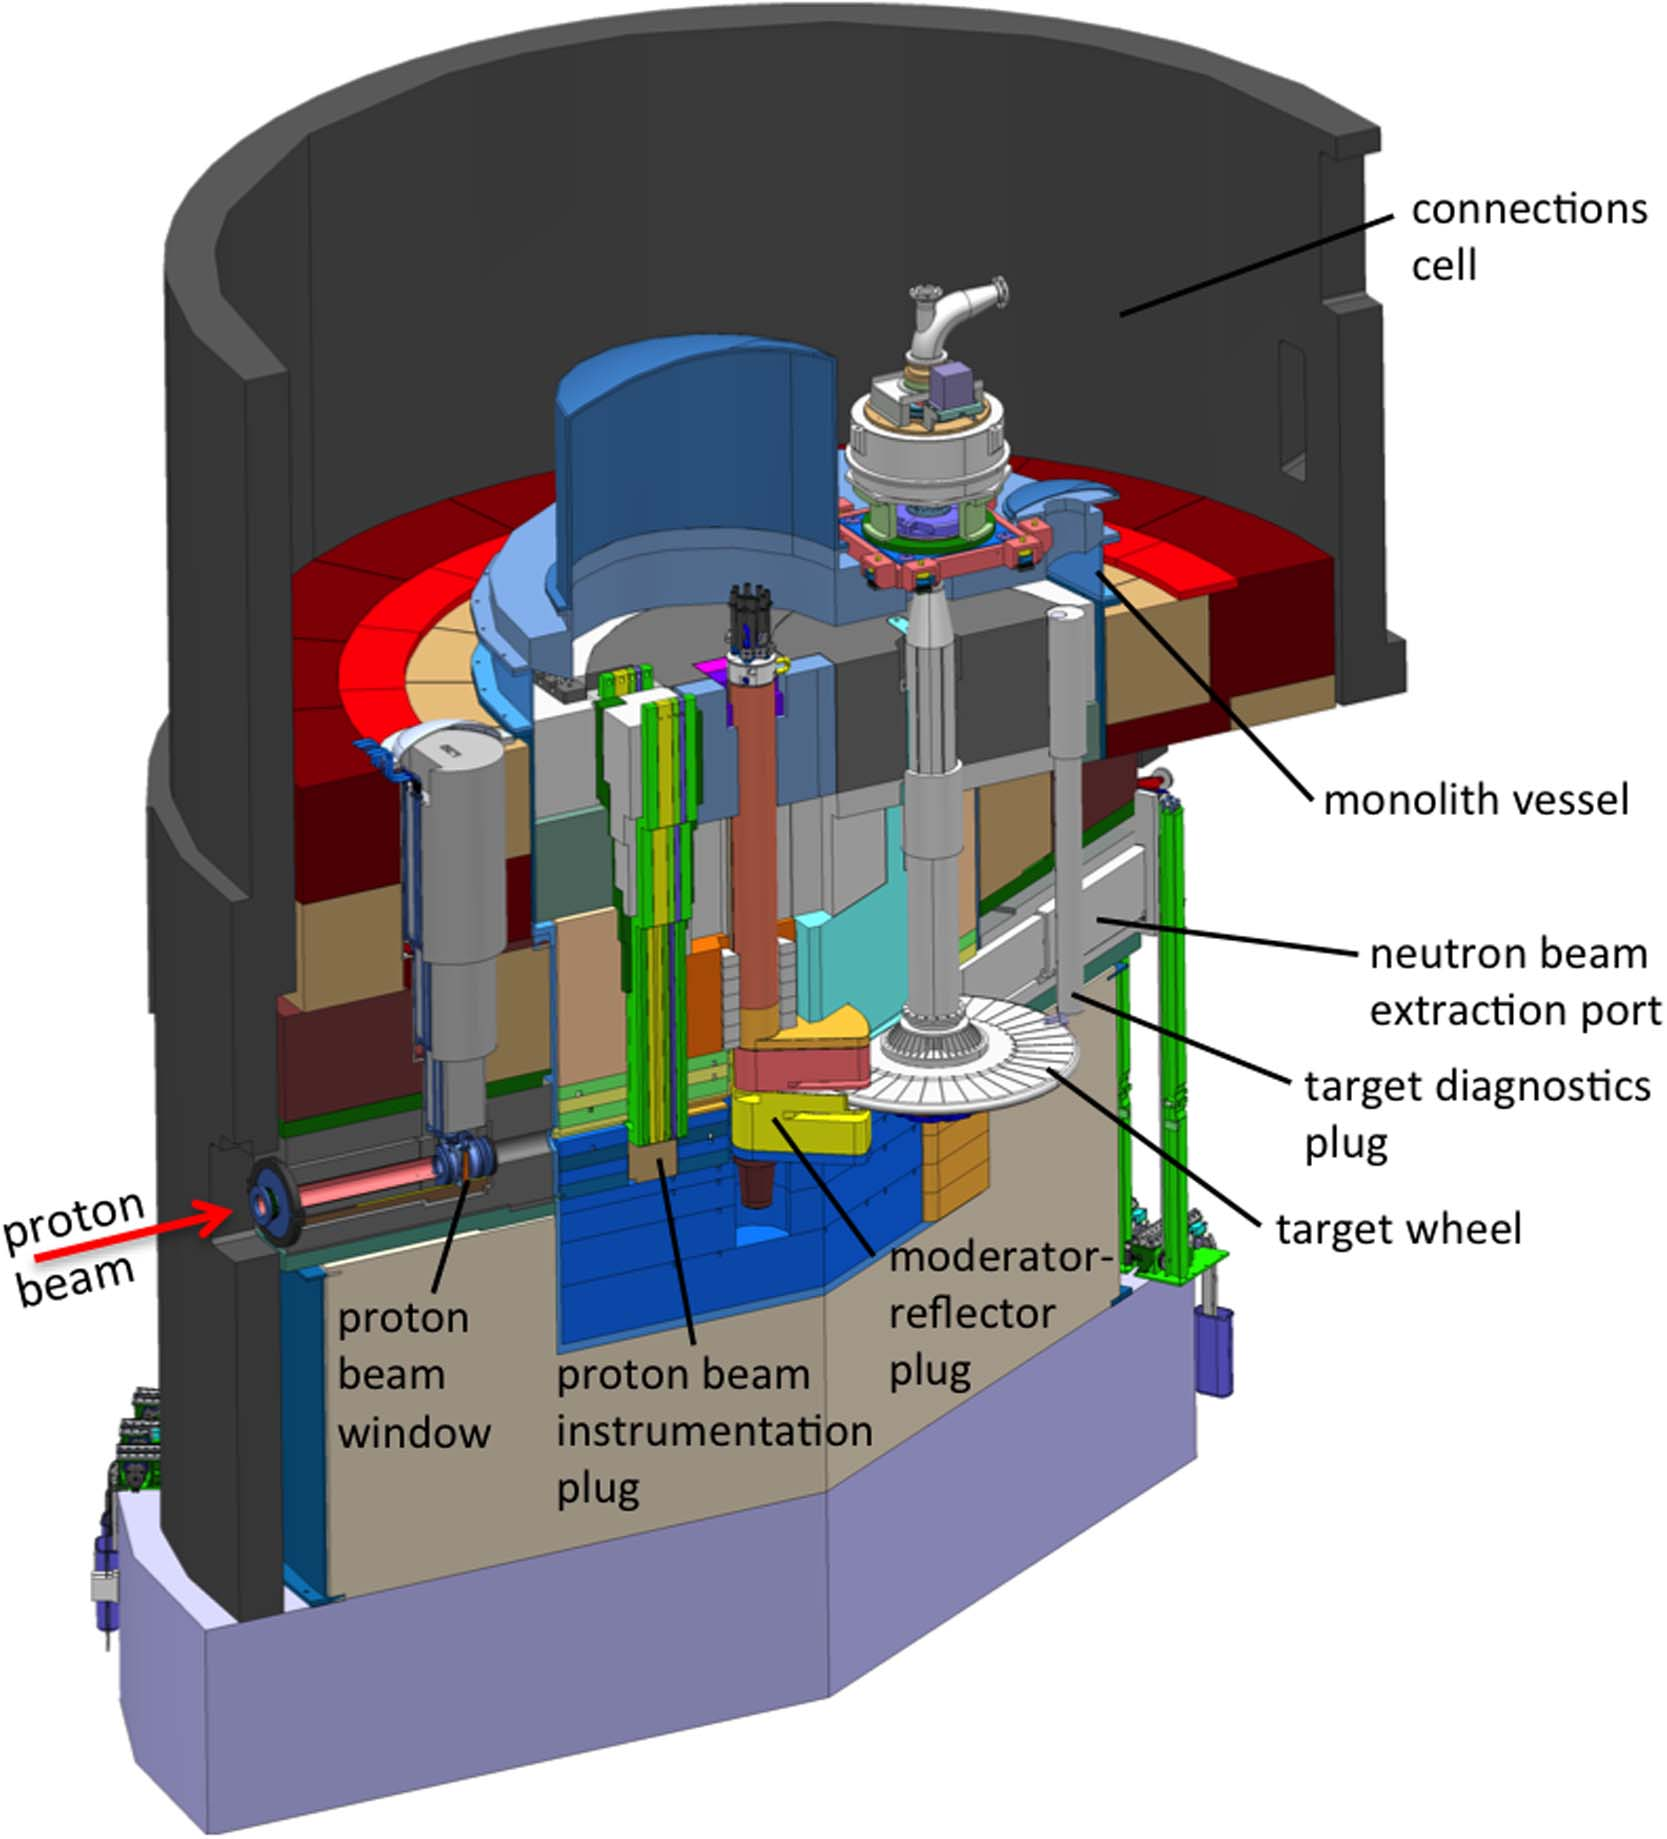
\includegraphics[width=\textwidth]{02_BeamDiag/figures/fig000_ESS_target_b}
	\end{center}
	\caption[The Tungsten target inside the monolith structure]{The Tungsten target inside the monolith structure.}
	\label{chap2:fig:target}
\end{figure}


  \section{Instruments}

  \begin{figure}[!ht]
  \begin{center}
    \begin{subfigure}[t]{0.45\textwidth}
      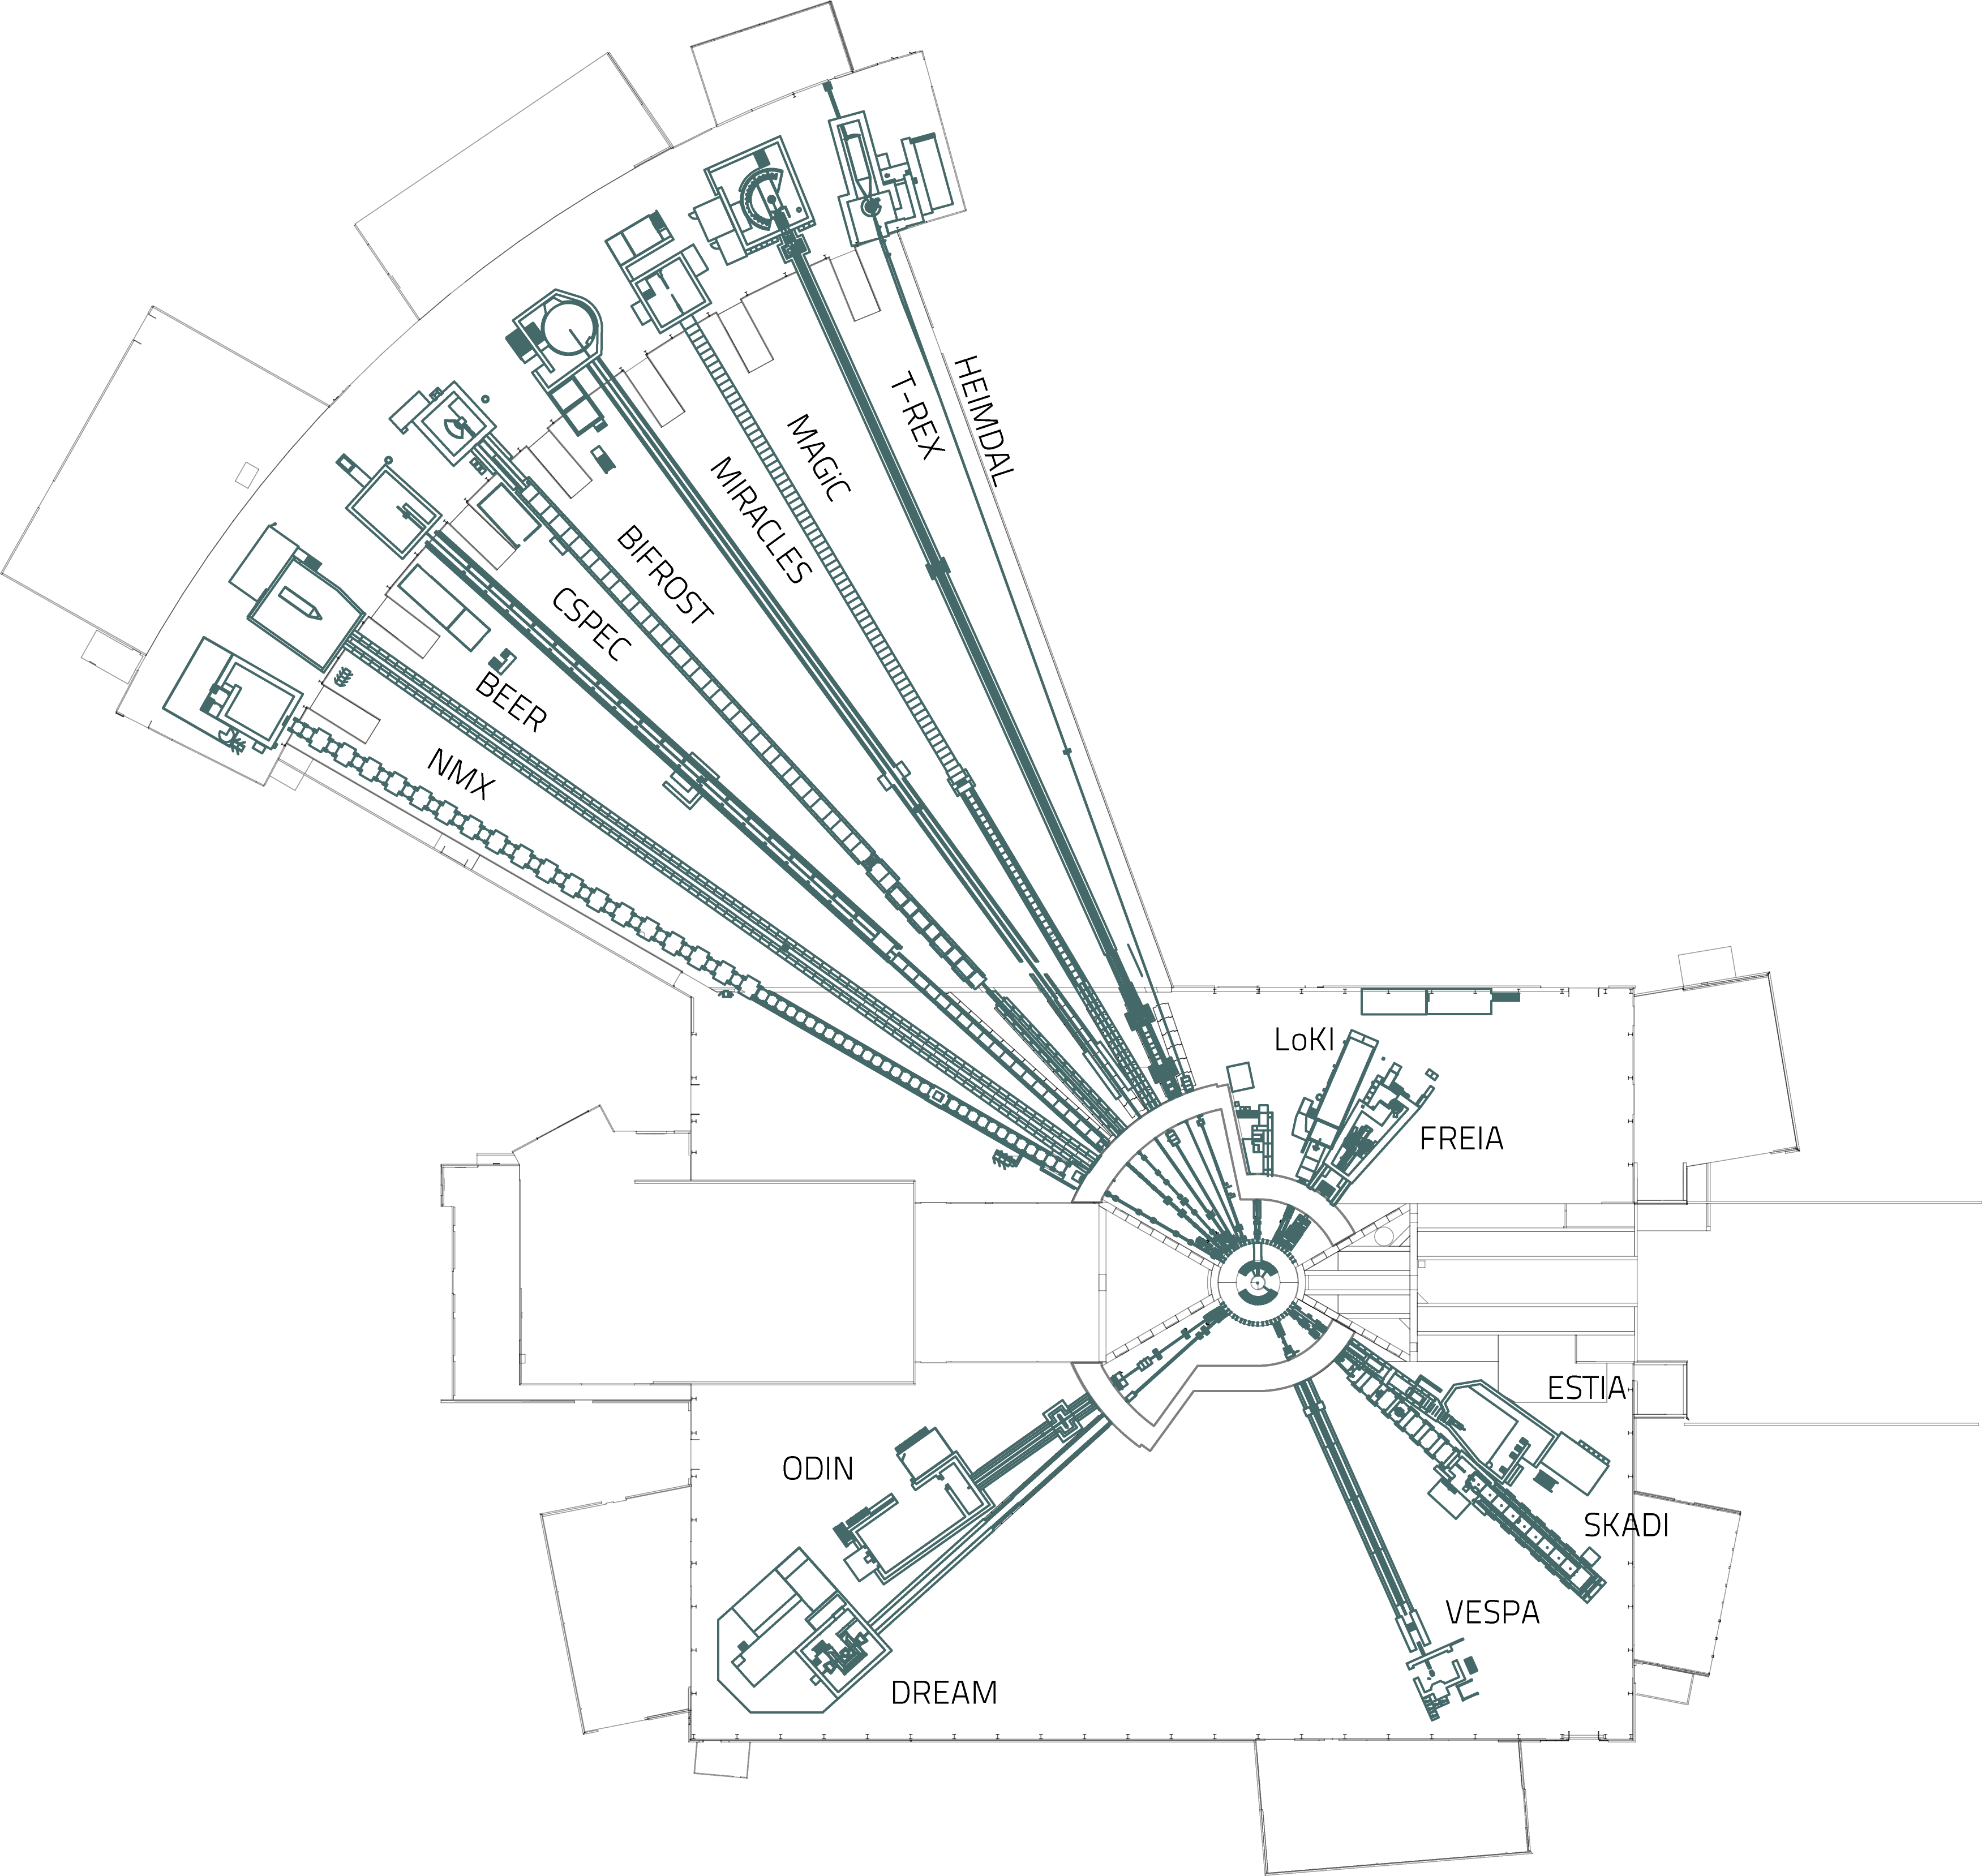
\includegraphics[width=\textwidth]{02_BeamDiag/figures/fig000_ESS_instruments}
      \caption{}
      \label{}
    \end{subfigure}
  \end{center}
  \caption[]{}
  \label{chap3:fig:ESS_instruments}
\end{figure}


  \section{Beam diagnostic overview}
  Beam diagnostics are used to ensure the proper functioning of the accelerator, the safety of persons and/or installations. They allow to measure the different beam characteristics such as current, position, beam losses, energy, profile, emittance etc. For each beam characteristic several methods can be considered, each of them having advantages and drawbacks. Beam diagnostics are at the crossroads of many areas of physics and electronics, belonging to the so-call transverse activities.

  The accelerating technologies are often complicated and quite expensive. In general, the size of the accelerator is reduced as much as possible, the space along the beam tube is often limited. The choice of diagnostics installed on a line must therefore be done carefully according to the expectations, neglecting diagnostics may be dramatic.

  The present section briefly\footnote{The proceedings of the CERN Accelerator School dedicated to beam diagnostics (2008 edition) is about 600 pages.} introduces different beam diagnostics frequently encountered on high intensity linear accelerators. Complete description of beam diagnostics can be found in books\cite{strehl2006}, Joint Universities Accelerator School \cite{juas2019} or CERN Accelerator School \cite{cas2019}.

  \subsection{Beam current monitor}
  % TODO: Référence
  The measurement of the beam current is perhaps the most basic information for an accelerator. Beam Current Monitors (\acrshort{bcm}) detect how many beam particle are passing through at specific positions on the accelerator. The transmission between the different accelerating blocks can be quantified.

  The BCM rely on very different method depending on the minimum value of the currents that should be achieved. For ESS, the beam current can be considered as high. Two common families of methods for measuring high currents are presented in this section.

  A Faraday cup (\acrshort{fc}) is a destructive method of current measurement. It can be seen as a beam dump, isolated from the accelerator ground, where the charges from the beam are collected by mean of a reading electronics. FC are often used in low energy parts of an accelerator (in LEBT for instance) because it can operate both as a current meter and beam dump. At high energy, the size and the complexity of the FC design increase a lot. A FC is usually inserted downstream the iris allowing a fine tuning of the current avoiding the injection of the beam into the entire accelerator. The critical part of the FC design is the cooling system that must be sufficiently efficient to dissipate the thermal power deposited by the beam. Repellers or suppressors electrodes or permanent magnets must be used to avoid any parasitic current due to secondary electron emissions during the impact of the beam particles.

  A beam consist of many charged particles moving together within bunches, more or less in the same direction; therefore a beam generates an electromagnetic field. The magnetic field can be used to measure the beam current in a completely non-invasive way by means of a current transformer (\acrshort{ct}). The beam can be seen as an one turn primary winding, and therefore the induced voltage measured on the secondary winding is proportional to the beam current. The measurement in the secondary winding is carried out by an active devices, an operational amplifier for instance, reducing the limitations of a passive measurement. Different implementations of current transformer exist depending on the requirement:
  \begin{itemize}
    \item Alternative Current Current Transformer (\acrshort{acct}): is the most common active transformer for pulsed beam.
    \item Fast Current Transformer (\acrshort{fct}): whose design is optimized for high-frequency current measurements, allowing bunch beam measurement for instance.
    \item Direct Current Current Transformer (\acrshort{dcct}): this type of transformer were developed to measure the DC component of a beam using a method similar to fluxgate sensor.
  \end{itemize}

  These diagnoses can be developed in-house or purchased directly off the shelf. On ESS, 18 ACCTs from Bergoz Instrument will be installed along the accelerator to measure the current. % \footnote{2 FCT are used in the MEBT}

  \subsection{Beam position monitor}
  % TODO: Référence

  \subsection{Beam loss monitor}
  Beam Loss Monitors (\acrshort{blm}) are mandatory diagnostics in all accelerator, and furthermore in high power accelerator facilities. When particles are lost in the accelerator, they will hit and pass through the beam tube elements producing various radiations. In an accelerator, BLM system primary goal is to guaranty the safety of the installation. Indeed, when the loss rates are high, the devices around the accelerator can be severely damaged.

  BLMs are very often connected to the machine protection system (\acrshort{mps}) allowing a fast shut down of the accelerator if the losses are too high. BLMs relies on a wide range of radiation detection techniques.

  At ESS two types of BLM are foreseen. The first loss monitors is based on ionization chambers (\acrshort{icblm}) \cite{Grishin:IBIC2017-WEPWC03}. These are the most common BLM types; icBLMs are widely used at CERN in \acrshort{lhc} \cite{HOLZER20122055}, SNS etc. In an icBLM, the losses ionize the gas in the chamber and a current is established between the electrodes. An icBLM has an high dynamic range, fast response and are cost effective.
  The second type of ESS BLM is completely new: the neutron Beam Loss Monitors (\acrshort{nblm}) \cite{Papaevangelou:HB2018-THA1WE04}.
  A nBLM is sensitive to fast neutrons and insensitive to radiations emitted by accelerator cavities. In fact, two nBLM types, based on Micromegas detector \cite{GIOMATARIS199629} were developed:
  \begin{itemize}
    \item A fast detector ($<\,50\,\mathrm{ns}$), sensitive to high losses allowing a very fast stopping of the beam.
    \item A slower detector ($<\,150\,\mathrm{\mu s}$), with a higher sensitivity, allowing a finely monitoring of the losses.
  \end{itemize}

  A total of 266 icBLMs, 42 slow nBLMs and 42 fast nBLMs will be installed along the accelerator.

  %\subsection{Beam emittance measurements}

  \section{Invasive beam profile measurements}
  \subsection{Interceptive screen}
  A luminescent screen provides a convenient way to measure profile since this diagnostic is simple to implement. The screen is put directly on the beam path using an actuator. When particles pass through the material, they partly deposit their energies, exciting the medium. During the de-excitation process, most of the energy is released to visible photon form. The intensity on the screen is proportional to the number of incident particles and their energy deposition. Therefore, it is possible to measure, with one camera, the profile directly in two dimensions by tilting the screen.

  The use of this diagnostic is strongly limited by the energy and intensity of the beam. At low energies and/or high current, the power to be dissipated can be locally considerable, reaching saturation and altering the screen properties. In general, a permanent decrease of the screen yield is observed \cite{Simon:IBIC2016-MOPG79} and in some extreme cases a deterioration of the screen surface.

  A concrete use of this type of diagnostics will be briefly presented in Chapter 4 with some experimental results.

  There is another type of intrusive diagnostics based on the optical transition radiation. The setup looks similar but the process behind is totally different. When a relativistic particle is subject to sudden variation of dielectric constant, i.e. between two media, transition photons are emitted with precise angles depending to the particle, its velocity and the angle of incidence. This method is well adapted for high relativistic accelerators such as $e^{-}$ \acrshort{linac} \cite{Nolle2009,Bolzon2013}.

  \subsection{Wire scanner}


  \subsection{SEM-Grid}
  A Secondary Electron EMission grid (SEM-Grid) or harp grid is a multichannel version of the SEM WS. Several wires are taut on a frame in the same direction at several positions. To avoid crosstalk due to secondary electrons, an electron repeller (wire or electrode) is often set around the wires. A second wire plane can also be placed in the transverse direction. Both grids are inserted in the beam tuned at low duty cycle and both profiles (X and Y) are measured in one shot. By using several SEM-grid successively the measurement of the transverse emittance is possible.

  However, the readout electronics of the secondary emission currents of all wires, is more complex due to the channel numbers. The number of wire must be chosen according to the resolution requirements on the beam sizes and positions. The wires must meet the same constraints as the wire scanner. The system is not necessarily more robust because if one wire breaks it may short circuit the other wires nearby.

  \section{Non-invasive beam profile measurements}
  \subsection{Laser wire profiler}
  For negative ion beams, a specific method, based on photo neutralization process, allows an almost (considering others beam losses) non invasive profile measurement. Photo neutralization works as follow: when a photon has a sufficient energy, it can strip off an electron of a negative ion.
  The photo neutralization cross section depends mainly on the energy of ions and on the wavelet of photons. With a dipole magnet free electrons are separated from the $H^-$ beam. Then, the electrons are collected and detected by a Faraday cup, a MCP or a semiconductor detector. The transverse profile is reconstructed by scanning the laser in the beam like a wire scanner.

  This kind of devices is popular on $H^-$ ion accelerators such as SNS and LINAC4. The method does not require any element passing through the beam. Therefore the laser wire scanners are very well suited for high intensity beams. The method requires an advanced laser system (typically $1064\,\mathrm{nm}$ Nd:YAG laser in $mJ$ range) \footnote{The laser can distributed on several measuring stations with optical fibers} as well as quite complicated optical setups.

  \subsection{Fluorescence Profile Monitor}
  % TODO: Mettre une image 
  Fluorescence Profile Monitors (\acrshort{fpm}) or Beam Induced Fluorescence (\acrshort{bif}) monitors are non-invasive diagnostic for transverse profile measurement. When the particles of the beam pass through the residual gas, they also can excite the residual gas. Fluorescence photons are emitted when the excited molecules return to their fundamental states.

  The fluorescence is a luminescent process that include the rapid  de-excitation (few tens of nanoseconds). The fluorescence occurs mainly with gases and each gas has its own emission spectra. Some gases have much larger effective cross-sections such as nitrogen, which is very often used. Fig. \ref{} shows a classic FPM assembly with an amplified detection readout and a gas injection system. In an ideal case, the vacuum chamber must have its light reflection capability as low as possible for reducing the background signal. This is commonly achieved by applying a black coating on the surface.

  However, detection is limited by several factors. The fluorescence photon is emitted within $4\pi$ angle, so the signal collected depends on the solid angle of the detector. The fluorescence cross section follows the Bloch equation and decreases very quickly with energy. FPMs are therefore preferred for low energy lines where the beam energy is low and the pressure high.  Otherwise, a FPM requires a gas injection system to increase the signal.

  This kind of detector will be installed almost everywhere at ESS except in the superconducting part where the very low pressure ($10^{-9}\,\mathrm{mbar}$)  and high beam energy no longer allows the profile measurement with FPM. Gas injection is not desired in the superconducting part.

  \section{Ionization Profile Monitor and summary}
  In the previous sections different methods for measuring the transverse profile has been presented. None of these methods may be able to measure the transverse profile in the superconducting part of ESS at nominal beam conditions. Wire scanners are very common devices but can not handle the beam power under the nominal conditions, moreover if one wires melt it could contaminate the surrounding cavities. Laser Wire scanners are very elegant solutions, on the other hand they can only work with negative ions. The very low pressures in the cryogenic part prevent the use of FPM and gas injection is not allowed at ESS.
  % TODO: Finish
  As superconducting accelerating part is the longest in terms of acceleration element, it would be harmful to leave this entire part without any transverse profile diagnostics.

  % TODO: IPM intro

  The method has been known since the late 1960s, but is continuously evolving with technological progress. First in terms of computing, nowadays computers are able to solve electromagnetic field equations, which greatly improves the understanding of IPMs making possible to understand and correct, various errors on measurement.
  Recently, the interest in semiconductor detectors has grown and an innovative IPM project using TimePix3 detectors is under development at \acrshort{cern} for the \acrshort{ps} \cite{Storey2015}. The first results are very promising \cite{Storey2017} and offer a new perspectives on IPM usages.

  The IPM method is now mature and used in several installations \cite{Krider1989,Wittenburg1992,Satou2006,Giacomini2011,Morris2011,egberts2012}.
  Fig. \ref{chap2:fig:IPM_3} shows 3 IPMs installed on 3 different accelerators. One can see directly that the design of an IPM is unique and tailor-made for its accelerator. This thesis deals about the development of IPMs for the superconducting part of the ESS accelerator. The different IPM technologies have been reviewed in order to select the most efficient one with respect to the ESS requirements.

  \begin{figure}[!ht]
  \centering
  \begin{subfigure}[t]{0.45\textwidth}
    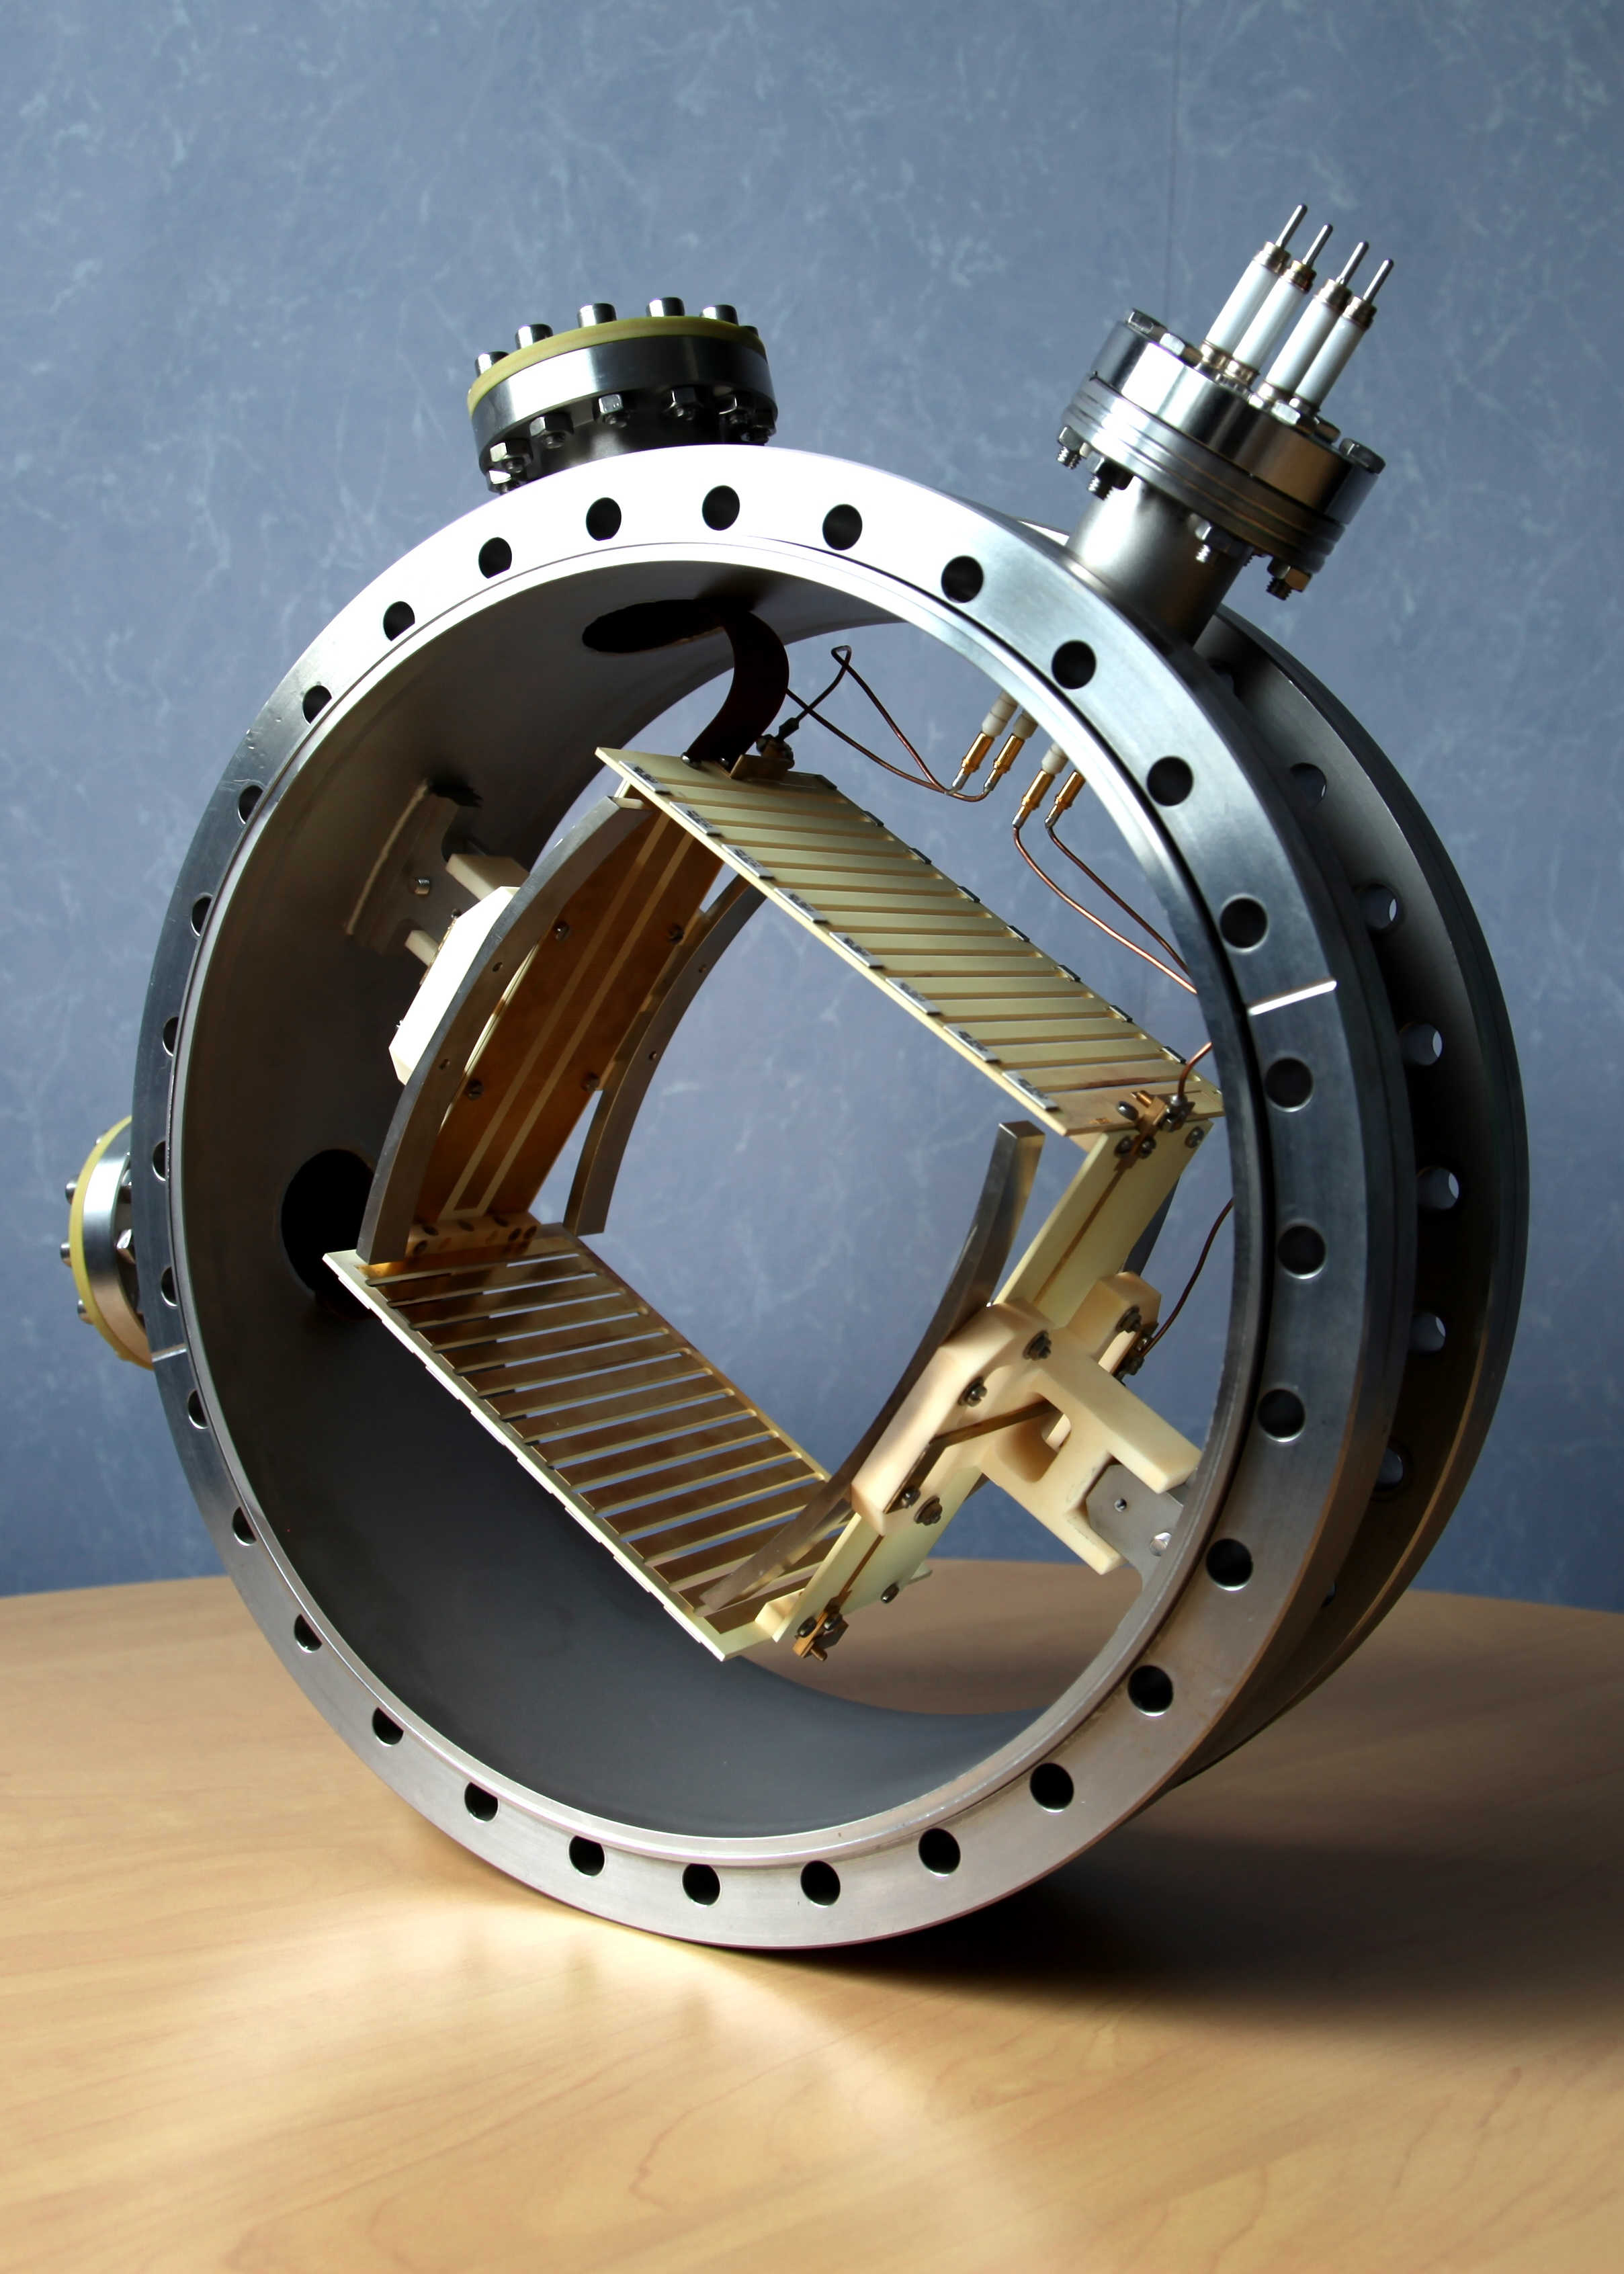
\includegraphics[width=\textwidth]{02_BeamDiag/figures/fig000_IPM_1}
    \caption[One of the IPM at IFMIF]{One of the IPM at IFMIF \cite{egberts2012}.}
    \label{}
  \end{subfigure}
  ~
  \begin{subfigure}[t]{0.45\textwidth}
    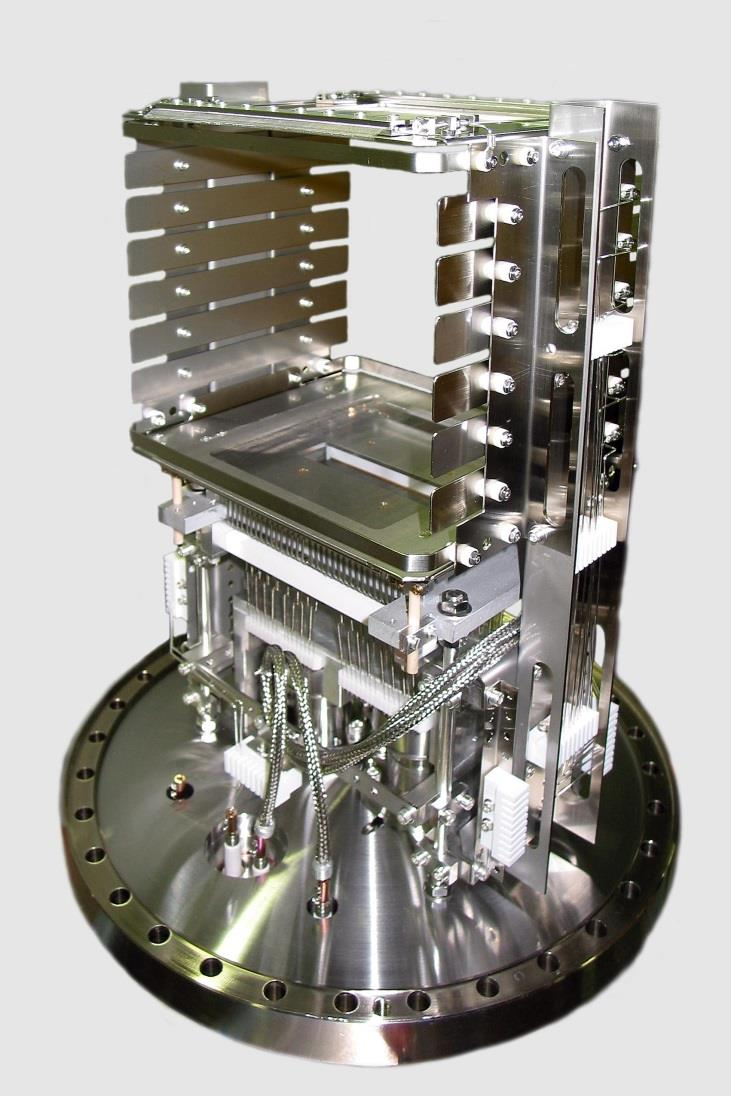
\includegraphics[width=\textwidth]{02_BeamDiag/figures/fig000_IPM_2}
    \caption[One of the IPM at GSI]{One of the IPM at GSI \cite{ForkJUAS}.}
    \label{}
  \end{subfigure}
  
  \begin{subfigure}[t]{1\textwidth}
    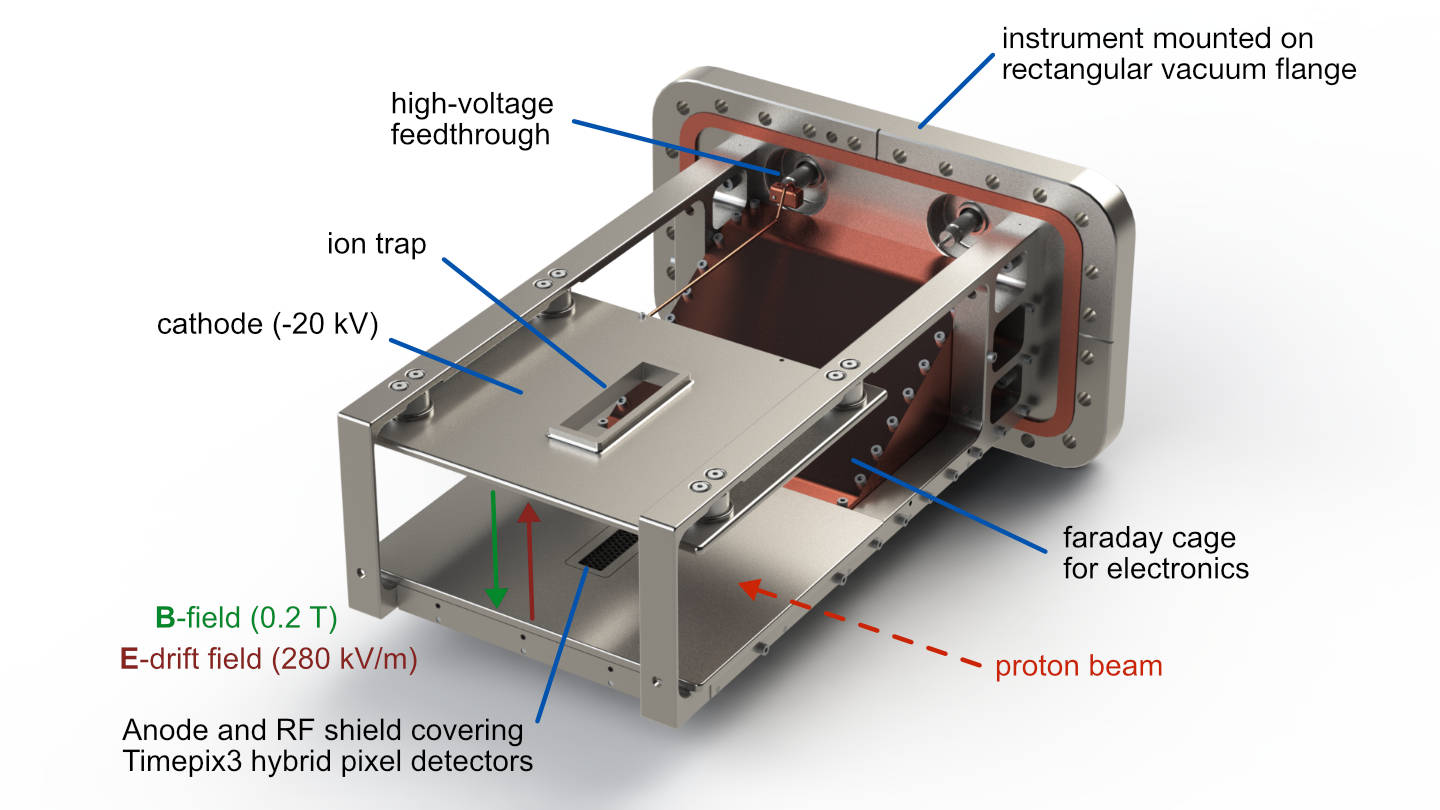
\includegraphics[width=\textwidth]{02_BeamDiag/figures/fig000_IPM_3}
    \caption[The future IPM for the PS]{The future IPM for the PS \cite{Storey2017}.}
    \label{}
  \end{subfigure}
  \caption[Three different implementations of IPMs on three different accelerators]{Three different implementations of IPMs on three different accelerators.}
  \label{chap2:fig:IPM_3}
\end{figure}


  \cleardoublepage
  \section*{Bibliography}
  \addcontentsline{toc}{section}{Bibliography}
  \label{ch2:bib}
  \printbibliography[heading=subbibliography]

\end{refsection}